Tektonická geomorfologie studuje tektonické tvary reliéfu a procesy, které tyto tvary utvářejí.

\section{Síla a napětí}
Na horniny v zemské kůře působí gravitační a tektonické síly, které v horninách vyvolávají \emph{napětí}. Napětí je přímo úměrné síle a nepřímo úměrné ploše, na kterou působí. Zapsat to tedy můžeme jako: 

\begin{equation}\label{eq:napeti}
	\text{napětí} = \text{síla}/\text{plocha}
\end{equation}

Celkové napětí lze rozdělit do tří na sebe kolmých komponent -- \emph{hlavních (principiálních) napětí}: $\sigma_{1}$ (největší), $\sigma_{2}$ (střední) a $\sigma_{3}$ (nejmenší napětí).
%\todo[inline]{vložit obrázek kostka napětí}.

\section{Tektonický režim}

Tektonické pohyby mohou reliéf ovlivňovat jak ve vertikálním i horizontálním směru. Při vertikálních posunech dochází ke změně nadmořské výšky, což vede ke změně energie reliéfu a tedy k urychlení odnosu a akumulace. Horizontální pohyby mění topografické uspořádání forem reliéfu, dochází ke změnám v půdorysu. 

Na základě uspořádání principiálních napětí můžeme rozlišit tři základní tektonické režimy:
\begin{itemize}
	\item Extenze
	\item Komprese
	\item Směrový posun
\end{itemize}

Při \emph{extenzi} dochází k roztahování zemské kůry a ztenčování, což se projevuje poklesovými zlomy. Při \emph{kompresním} režimu dochází ke zkracování zemské kůry. To vede ke vzniku vrás, přesmyků či příkrovů. U směrových posunů dochází k pouhému posouvání ker zemské kůry podél sebe v opačném směru. Pokud je horizontální posun kombinován i s vertikální složkou hovoříme o \emph{transpresním}, respektive \emph{transtenzním} režimu.

%\todo[inline]{obrázek zlomy, napetove rezimy}

Tektonické pohyby rozlišujeme podle stáří. \emph{Paleotektonické} pohyby se projevují pouze ve struktuře. Reliéf mohou ovlivňovat jen pasivně. {Neotektonické} pohyby se projevují v současném reliéfu. Do neotektonických pohybů patří i současné pohyby zemské k ůry.

Tektonické pohyby se rozlišují i podle toho, zda je při nich narušena spojitost hornin. \emph{Plikativní (duktilní, vrásové)} pohyby jsou spojité. Jedná se o plastickou deformaci hornin a není tak narušena jejich spojitost. \emph{Disjunktivní (zlomové)} pohyby jsou nespojité, dochází k rozpojení hornin, průběžnost vrstev je narušena.

\section{Zlomy}
Jako \emph{zlom} (\enquote{fault}) se běžně označuje plocha, diskontinuita, v horninovém tělese, podél které došlo k pohybu -- dislokaci. Ve skutečnosti je zlom trojrozměrné těleso, avšak jeho třetí rozměr (tloušťka) je zanedbatelný. Zlom vymezují \emph{zlomové plochy}, na kterých bývají stopy pohybu -- \emph{striace}. Zlom odděluje dva bloky (kry) zemské kůry. Pokud je zlom ukloněn, kra nad zlomem se označuje jako \emph{nadložní} (\enquote{hanging-wall}) a kra pod zlomem jako \emph{podložní} (\enquote{foot-wall}).

Podle smyslu pohybu bloků dělíme zlomy na (Obr. \ref{fig:zlomy}):
\begin{itemize}
	\item Poklesové (normální)
	\item Přesmyky (reverzní zlomy)
	\item Horizontální posun
\end{itemize}

\begin{figure}[h]
	\centering
	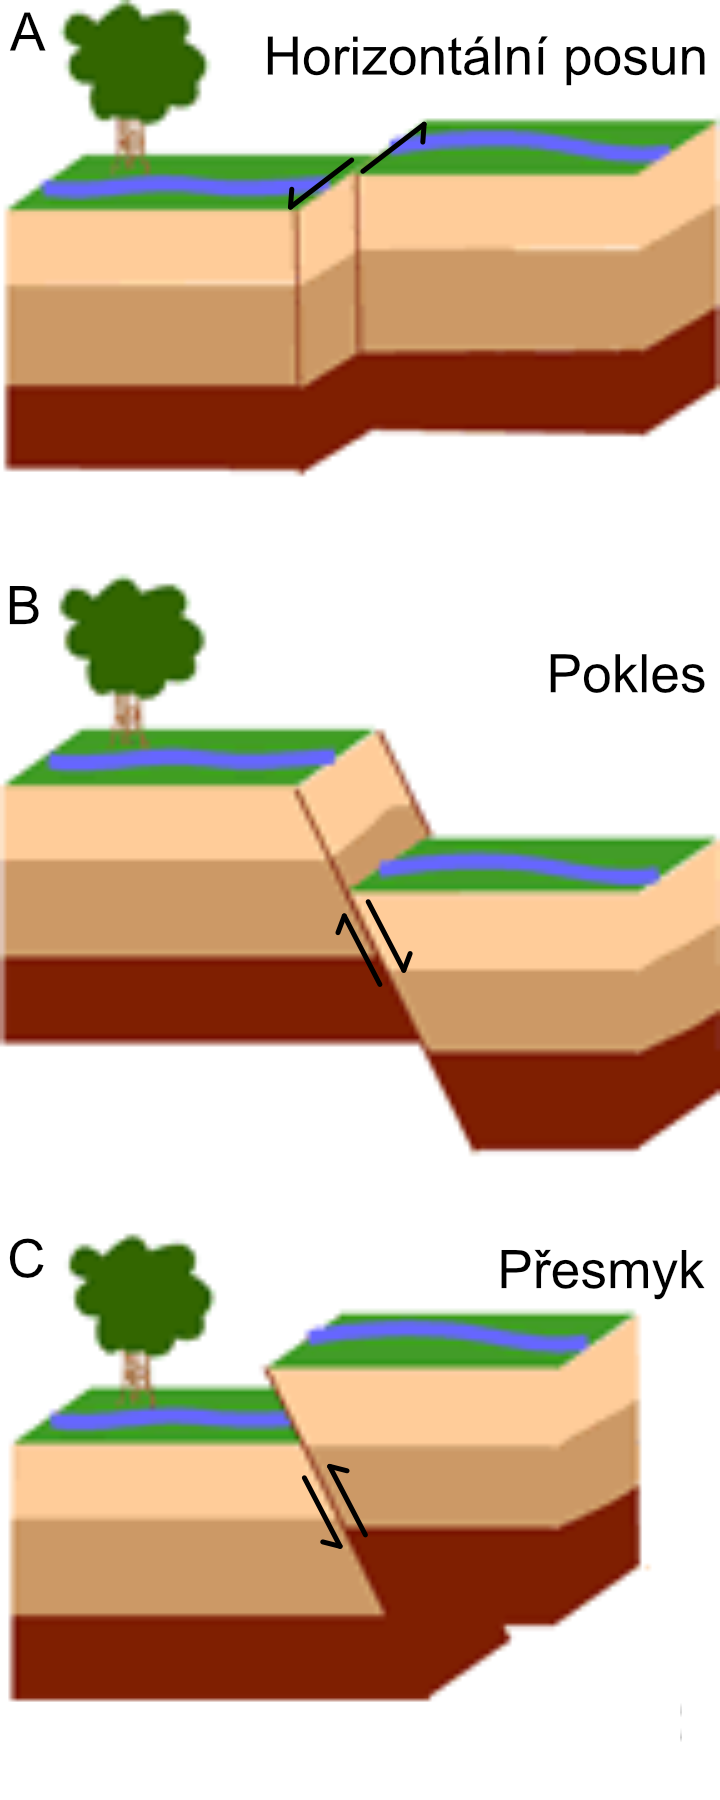
\includegraphics[width=0.8\linewidth]{obrazky/tectonic/zlomy}
	\caption{Typy zlomů. A horizontální posun (levostranný), B pokles, C přesmyk (upraveno podle USGS, volné dílo).}	
	\label{fig:zlomy}
\end{figure}

\subsection{Typy zlomů}
\subsubsection{Horizontální posun}
\emph{Horizontální (směrný) posun} (Obr. \ref{fig:zlomy}A) je zlom charakteristický horizontálním posunem bloků ve směru paralelním k průběhu zlomu. Horizontální posuny velkých rozměrů se nazývají transformní zlomy (viz desková tektonika).

Na základě směru posunu dělíme horizontální posun na pravostranný (dextrální) a levostranný (sinistrální). Orientaci zlomu poznáme jednoduše. Postavíme se čelem ke zlomu a směr určíme podle pohybu protilehlé kry vůči našemu stanovišti Při pravostranném zlomu se protilehlá kra hnula doprava, u levostranného zlomu je tomu naopak. 

Horizontální posuny jsou seismicky nejaktivnější typ zlomů. Typickým příkladem transformního zlomu je zlom San Andreas (Obr. \ref{fig:san_andreas}).

\begin{figure}
	\centering
	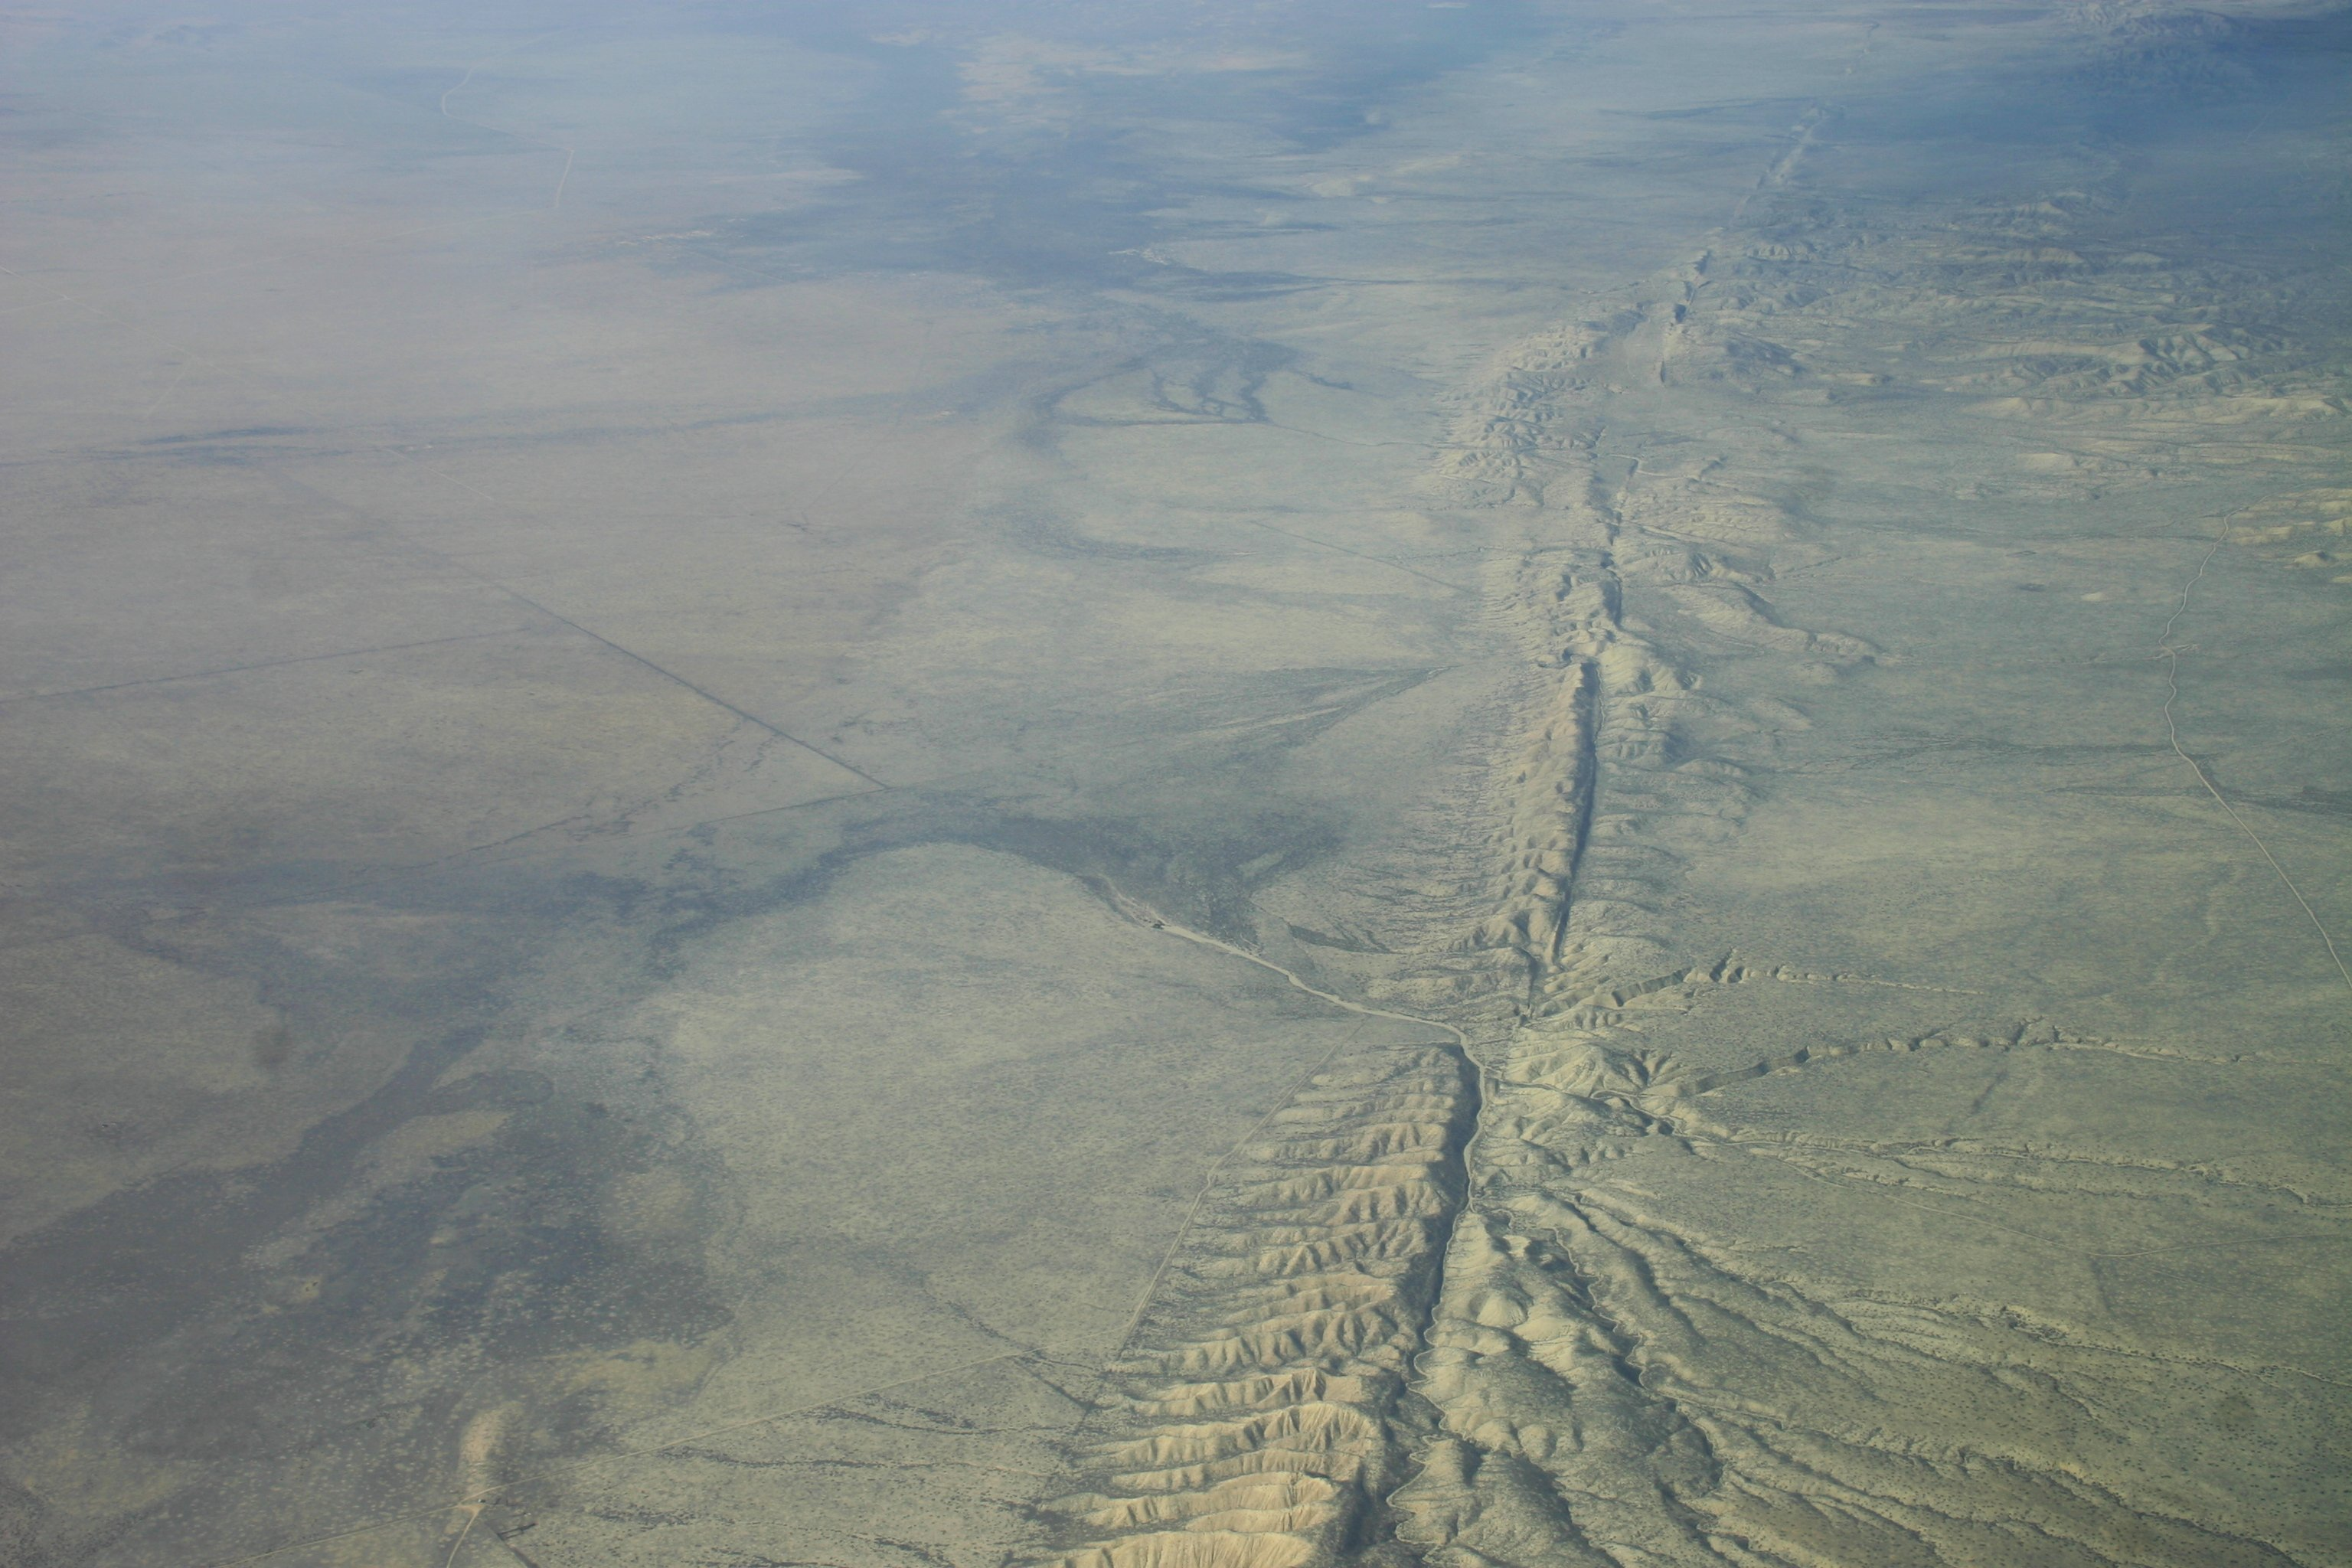
\includegraphics[width=1\linewidth]{obrazky/tectonic/san_andreas}
	\caption{Pohled na zlom San Andreas, Carrizo Plain (autor Ian Kluft, CC-SA 4.0)}
	\label{fig:san_andreas}
\end{figure}

Horizontální posuny se v reliéfu projevují víceméně přímočarými liniemi, jelikož jsou převážně vertikální. Směrným posunem dochází k ohybům vodních toků. 

Zřídkakdy je průběh zlomu zcela rovný. V místech ohybů tak dochází k lokální extenzi \emph{(transtenze)} nebo kompresi \emph{(transprese)}. Extenzí vznikají poklesy, tzv. \emph{pull apart pánve}. Při kompresi dochází výzdvidhu zemské kůry a vzniku \emph{kompresních hřbetů}.

\subsubsection{Pokles}
\emph{Poklesové zlomy} (\enquote{normal fault}) (Obr. \ref{fig:zlomy}B, \ref{fig:pokles}) jsou důsledkem extenze zemské kůry. Jsou charakteritické velkým sklonem (\SIrange{50}{60}{\degree}) vzhledem k povrchu. Poklesává nadložní kra. Tedy podložní kra je v ve vyšší pozici oproti nadložní kře. 

Velké poklesové zlomy mají \emph{listrický} tvar. To znaméná, že jsou konkávně zakřivené. S hloubkou se jejich sklon zmenšuje někdy až do horizontální pozice. V případě zakřivených poklesových zlomů vznikají oproti nim sekundární poklesové zlomy, které mají opačný směr sklonu a smysl pohybu. Označují se jako tzv. \emph{antitetické zlomy}.

\begin{figure}
	\centering
	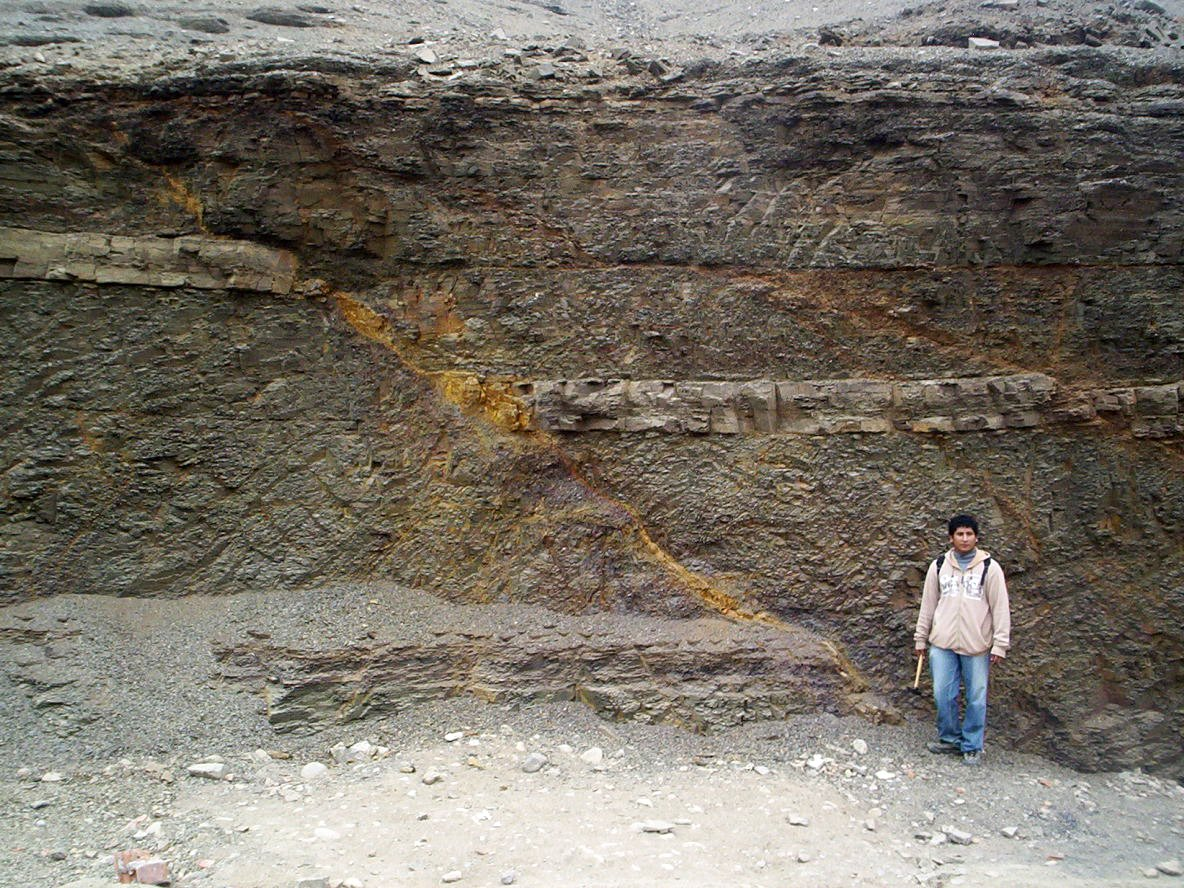
\includegraphics[width=1\linewidth]{obrazky/tectonic/pokles}
	\caption{Příklad normálního (poklesového zlomu) v v souvrství La Herradura. Lokace Morro Solar Lima, Peru (autor: Miguel Vera León)}
	\label{fig:pokles}
\end{figure}

\subsubsection{Přesmyk}
\emph{Přesmyk} (\enquote{reverse fault}) (Obr. \ref{fig:zlomy}C) je důsledkem komprese (zkracování) zemské kůry. Se zkracováním narůstá mocnost kůry. Přesmyky jsou charakteristické menším sklonem, který se pohybuje okolo \SI{30}{\degree}. Nadložní kra se nasouvá na podložní. Nadložní kra se tak nachází ve vyšší pozici než kra nadložní. 
Přesmyky dělíme na kerné, které jsou čistou střižnou deformací, a vrásové, které vznikly přetrhnutím jednoho ramena vrásy.

\subsubsection{Násun}
\emph{Násun} (\enquote{thrust}) je specifickým typem přesmyku. Úklon násunu je zpravidla velice mírný až subhorizontální. 

\subsection{Projev zlomů v reliéfu}
\subsubsection{Zlomový svah}
Nejběžnějším projevem vertikálního pohybu na zlomech je \emph{zlomový sráz, stupeň} (\enquote{fault scarp}) (Obr. \ref{fig:faultscarp}). Zlomové stupně často vznikají při zemětřeseních (koseismické pohyby). Dlouhodobou kumulací pohybů při zemětřeseních, případně vytrvalým výzdvihem jedné kry (resp. poklesem druhé), tzv. interseismickými pohyby, se vyvíjí \emph{zlomový svah}. Okraje pohoří vyzdvižených podél zlomů jsou charakteristické tzv. facetami. Jsou to trojúhelníkové nebo lichoběžníkové plochy vzniklé rozčleněním a přemodelováním zlomových svahů erozí (obr. \ref{fig:facety}). Jejich sklon je nižší, než sklon zlomových svahů. Typicky se pohybuje mezi \SIrange{25}{35}{\degree}.

\begin{figure*}[h]
	\centering
	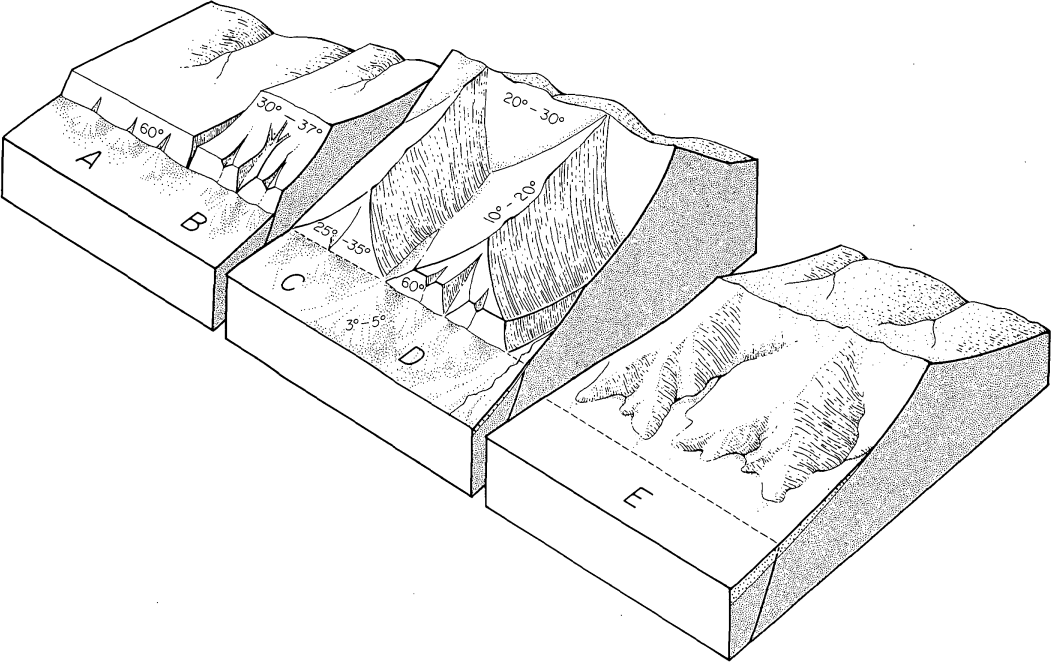
\includegraphics[width=1\linewidth]{obrazky/tectonic/facety}
	\caption{Ukázka vývoje zlomového okraje pohoří a vzniku facet. A: čerstvý zlomový svah; B: postupné zařezávání vodních toků (strže), přemodelování zlomového stupně; C,D: vyvinutá údolí a facety, opakovaný nebo intenzivní výzdvih udržuje zlomový svah (D); E: dlouhé období tektonického klidu, postupná denudace (převzato z \textcite{wallaceGeometryRatesChange1978})}
	\label{fig:facety}
\end{figure*}




\begin{figure*}[h]
	\centering
	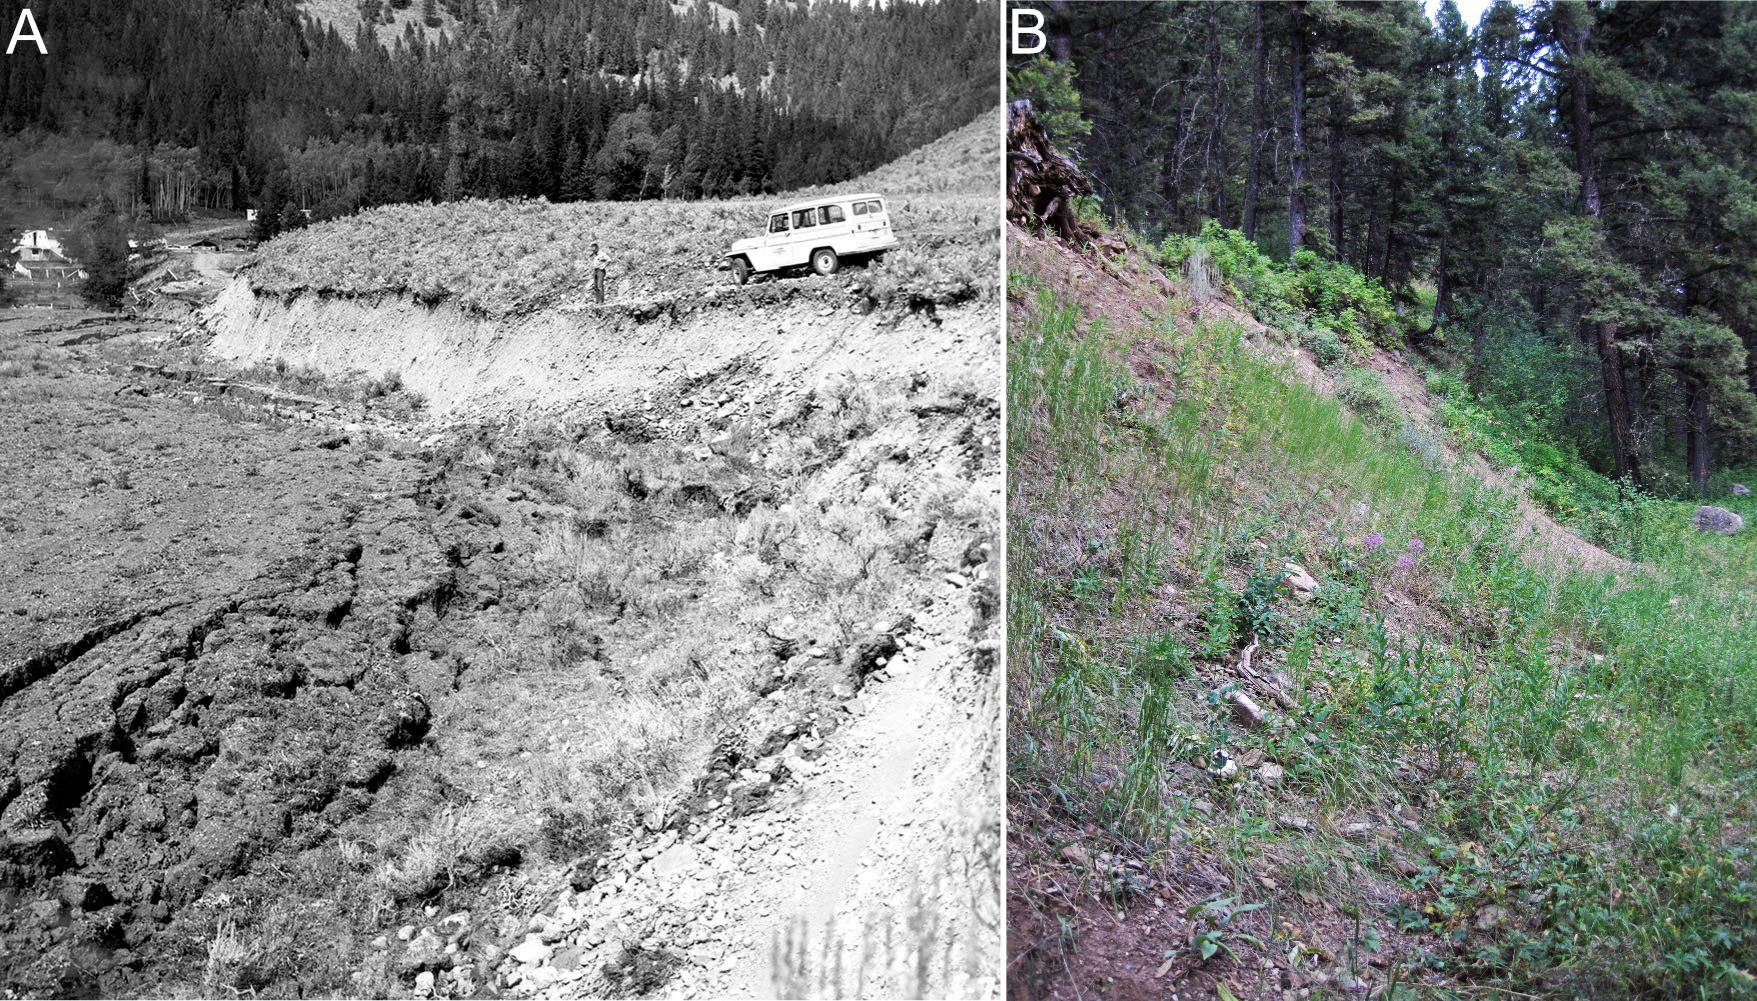
\includegraphics[width=1\linewidth]{obrazky/tectonic/fault_scarp}
	\caption{Zlomový sráz, který vznikl při Yellowstonském zemětřesení v roce 1959. A fotografie pořízená těsně po události (autor J. R. Stacy, USGS, volné dílo/Public Domain). B Stupeň již částečně zhlazený difuzními procesy o 59 let později (autor James St. John, CC BY 2.0).}
	\label{fig:faultscarp}
\end{figure*}

Rychlost degradace zlomového srázu je daná především pevností dané horniny. Rychleji bude degradovat stupeň vzniklý jen nezpevněných sedimentech, než v pevných horninách. Dalším faktorem je intenzita exogenních procesů. 

Rychlost pohybu na zlomu ovlivňuje podobu zlomových svahů. Zlomové svahy na poklesových zlomech s rychlým pohybem mají výrazné a málo degradované facety, údolí členící zlomový svah jsou úzká a hluboce zařezaná. Při pomalém pohybu na zlomu jsou facety degradované, údolí zařezávající se do podložní kry jsou široká a v předpolí se nachází velké, mírně ukloněné výplavové kužely, do kterých je zaříznutý vodní tok. 

Pohybem na zlomu může dojít k tomu, že na jedné straně zlomové plochy se nacházejí méně odolné horniny, než na straně druhé. Jelikož eroze bude postupovat rychleji v méně odolných horninách, může vzniknout nový svah tzv. \emph{svah na zlomové čáře}. Podle orientace nového svahu vůči zlomu jej dělíme na tzv. resekventní svah, který má stejnou orientaci jako původní zlomový svah, a obsekventní svah s opačnou orientací.

\subsubsection{Hrástě a prolomy}
V soustavě paralelních zlomů vznikají hrástě a prolomy. \emph{Hrásť} (\enquote{horst}) je protáhlá vyvýšenina. Jedná se o kru, která je vůči svému okolí nejvyšší. Hrástě mohou vznikat výzdvihem kry -- je tedy omezena přesmyky, které mají úklon pod vyzdviženou kru. Tento typ hrástí označujeme jako \emph{automorfní hrástě}. Hrástě, které vznikly poklesem okolních ker (tedy její omezení je poklesovými zlomy), se nazývají \emph{xenomorfní hrástě}.

Protáhlé sníženiny omezené poklesovými zlomy se nazývají \emph{prolomy} (\enquote{graben}). Prolomy jsou také označovány jako \emph{riftová údolí}.  Pokud je sníženina omezená jedním velkým listrickým zlomem na jedné straně a případnými kompenzčními antetickými zlomy na druhé, hovoříme o tzv. \emph{polo-prolomech} (\enquote{half-graben}). V prolomech a  poloprolomech se ukládá velké množství sedimentů z okolních elevací. Mocnost sedimentů může být enormní - až v řádu kilometrů.

Taktéž může nastat, že se jedna kra ukloní -- na jedné straně dojde k jejímu poklesu, na opačné pak k výzdvihu. 

\subsubsection{Projevy horizontálních pohybů}

Horizontální pohyby mohou ovlivnňovat reliéf pasivně tím, že bude docházet k selektivní erozi podél tektonicky oslabených hornin. Aktivní ovlivnění reliéfu horizontálními pohyby se projevuje v dislokaci geomorfologických a jiných krajiných prvků. Dochází tak ke zmenám v půdorysu. Nejvíce je to patrné na geomorfologických sítích (vodní toky).

Jedním z důsledků horizontálního posunu může být například posunutí průběhu hřbetů a údolí.

\subsubsection{Příkrovy}
\emph{Příkrovy} (\enquote{nappes}) jsou rozsáhlá tělesa přesunutá podél násunových zlomů na vzdálenost minimálně 5 km. Běžně se jedná ale o přesuny až na vzdálenost desítek kilometrů. Příkrov (přesunuté těleso) se označuje jako \emph{alochton}, stabilní podloží je \emph{autochton}.

\section{Pukliny}
\emph{Pukliny} (\enquote{joints}) jsou diskontinuity podél kterých nedošlo k pohybu nebo byl neznatelný. Pukliny jsou nejrozšířenějším typem diskontinuit. Jejich klasifikace je založená na základě celé řady kritérií (tvar, velikost, frekvence,...). Pukliny mohou být systematické (systém subparalelních puklin) a nesystematické (nepravidelné, zakřivené). 

Pukliny mohou pasivně ovlivňovat vývoj reliéfu, jelikož to jsou místa oslabení horninového masivu. Může jimi například snadno pronikat voda a urychlovat zvětrávání a erozi horniny. Pěkně je tento vliv puklinových systémů na reliéf vidět u pískovcových skalních měst. Soutěsky se vyvíjejí podél jednotlivých puklinových systémů, na kterých koncentruje erozní činnost.

\section{Vrásy}
\emph{Vrásy} (\enquote{folds}) vznikají duktilní deformací hornin. Jedná se o spojité tektonické struktury. K vrásnění dochází při kompresním režimu, kdy se ohybem planárních struktur hornin (např. vrstev) zkracuje zemská kůra. Jednoduché prohnutí vrstev je označováno jako \emph{flexura}. Narozdíl od vrás mohou flexury vznikat i v extenzním režimu. Vrásy jsou často ve spojení se zlomy.

Rozlišujeme \emph{antikliálu}, což je část, která je vyklenutá vzhůru a \emph{synklinálu}, jejíž vyklenutí je směrem dolů. Část, která spojuje antiklinálu a synklinálu, se nazývá \emph{rameno vrásy} nebo také křídlo vrásy.

\begin{figure}[h]
	\centering
	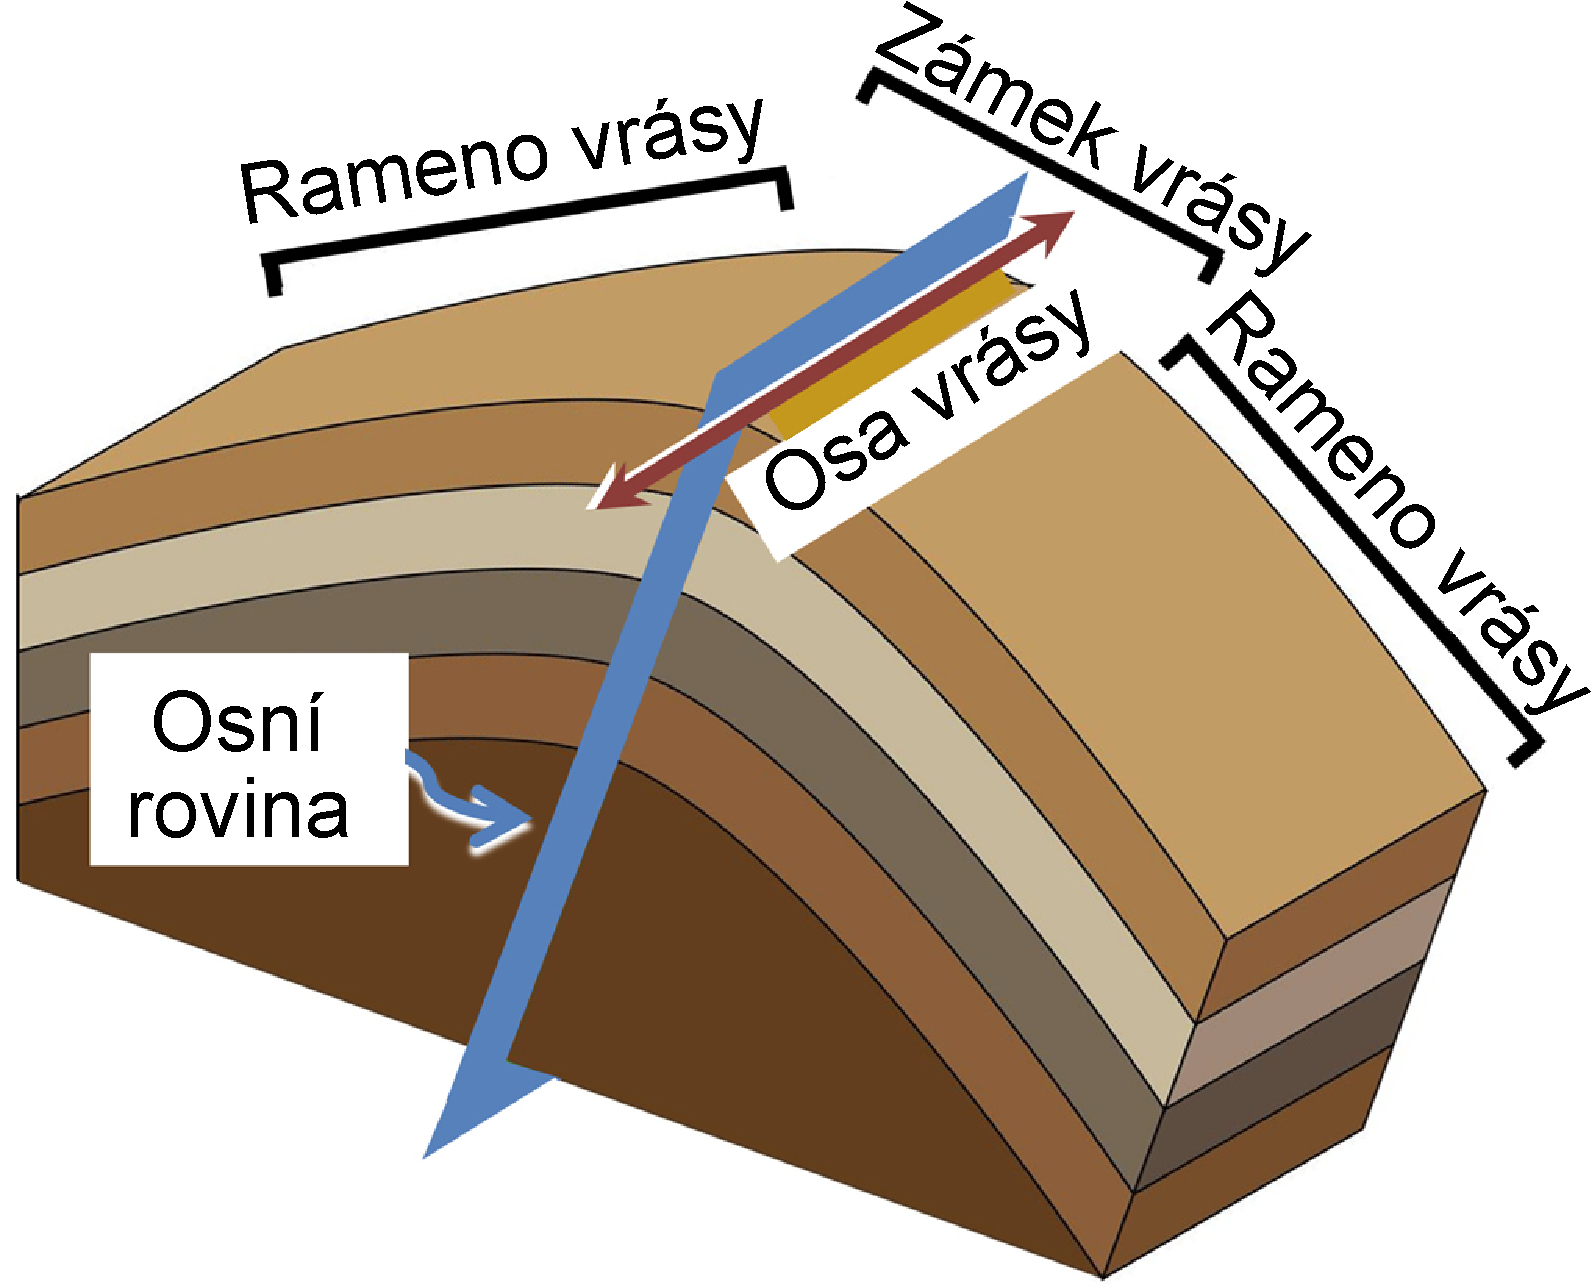
\includegraphics[width=\linewidth]{obrazky/tectonic/fold_parts}
	\caption{Části vrásy (Upraveno podle Brews Ohare, CC BY-SA 3.0)}
	\label{fig:foldparts}
\end{figure}

Vrásy dělíme podle osní roviny na:

\begin{itemize}
	\item vzpřímené
	\item ukloněné
	\item převrácené
	\item ležaté
\end{itemize}

Další dělení vrás je podle sevřenosti jejich ramen:
\begin{itemize}
	\item rozevřené
	\item otevřené
	\item sevřené
	\item zavřené
	\item izoklinální
\end{itemize}

Vrásy také můžeme rozdělit na symetrické a nesymetrické. V případě prohnuté osy vrásy hovoříme o tzv. brachyantiklinálách a brachysynklinálách.

\subsection{Izometrické vrásy}
Specifickou formou vrás jsou tzv. izometrické vrásy. Jedná se o vrásové struktury, které nejsou protažené jedním směrem. 

Synklinální sníženiny oválného až kruhovitého půdorysu se nazývají \emph{pánve}. Výraznost pánevních oblastí je daná velikostí prohnutí vrstev (čím větší, tím je pánve výraznější) a na míře zaplnění pánve sedimenty. Na okrajích pánví lze nalézt asymetrické hřbety -- kuesty (viz dále). 

Vyklenutím hornin vzhůru vznikají \emph{klenby}. Jedná se o velká tělesa oválného až kruhového půdorysu. Klenby mohou vznikat intruzí magmatu mezi vrstevní plochy, což způsobuje vyklenutí nadložních vrstev. V takovém případě se jedná o \emph{klenby s krystalickým jádrem}. \emph{Sedimentární klenba} nemá krystalické jádro, vzniká prostým prohntím sedimentárních hornin v důsledku bočních tlaků. K vyklenutí může dojít také kvůli intruzím solných diapirů působením hydrostatických nebo tektonických tlaků. Vznikají tak \emph{solné klenby}. 

\subsection{Projev vrás v reliéfu}
Vztah mezi zvrásněným podložím a georeliéfem může nabývat celé řady podob. Vrásy vytvářejí \emph{vrásová pohoří}. Vazba mezi reliéfem a strukturou může být \emph{přímá} -- v místě antiklinály se nachází hřbet a v místě synklinály údolí. 

Jednoduchá vrásová pohoří vznikají, když vrásy mají jen minmálně zvlněné osy. Tvoří pak paralelně probíhající soustavu hřbetů a údolí. Takovýto typ pohoří je označován jako Jurský typu reliéfu (podle pohoří Jura ve Švýcarsku). Kromě pohoří Jura je příkladem Zagros v Íránu (Obr. \ref{fig:zagros}). 

Při značném zvlnění os vrás, vznikají složitá vrásová pohoří tvořená soustavou brachyantiklinál a brachysynklinál. Tento typ se označuje jako Apalačský podle pohoří v USA (Obr. \ref{fig:apalachian}).

\begin{figure}[h]
	\centering
	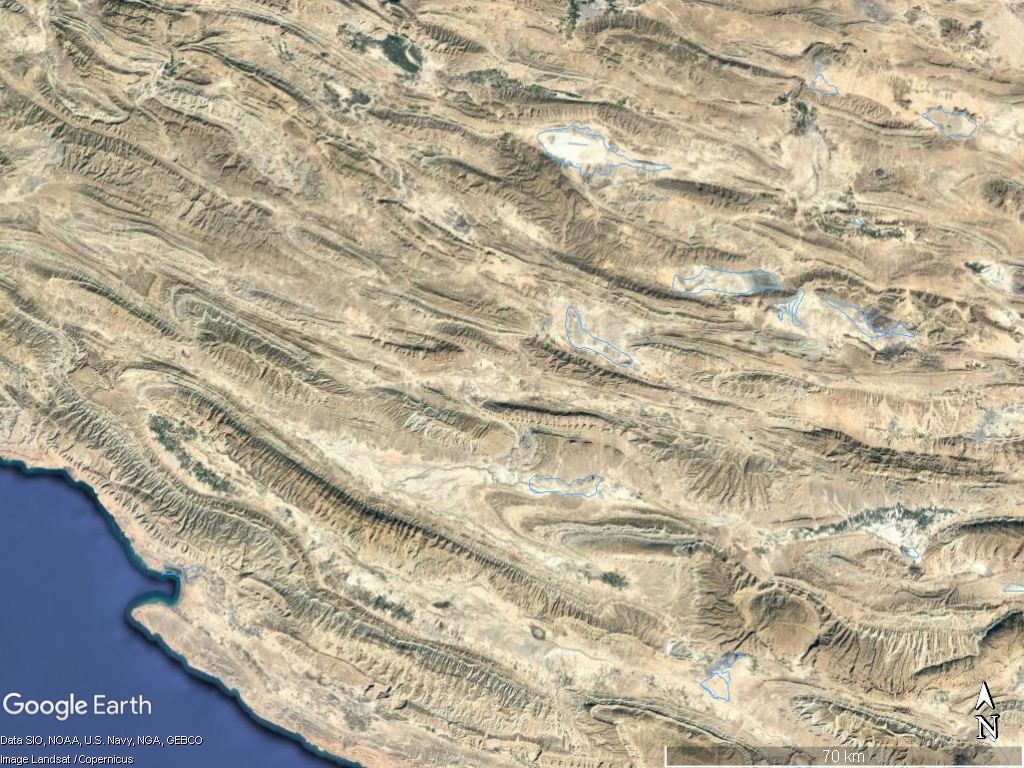
\includegraphics[width=1\linewidth]{obrazky/tectonic/zagros}
	\caption{Pohoří Zagros (zdroj Google Earth)}
	\label{fig:zagros}
\end{figure}

\begin{figure}[h]
	\centering
	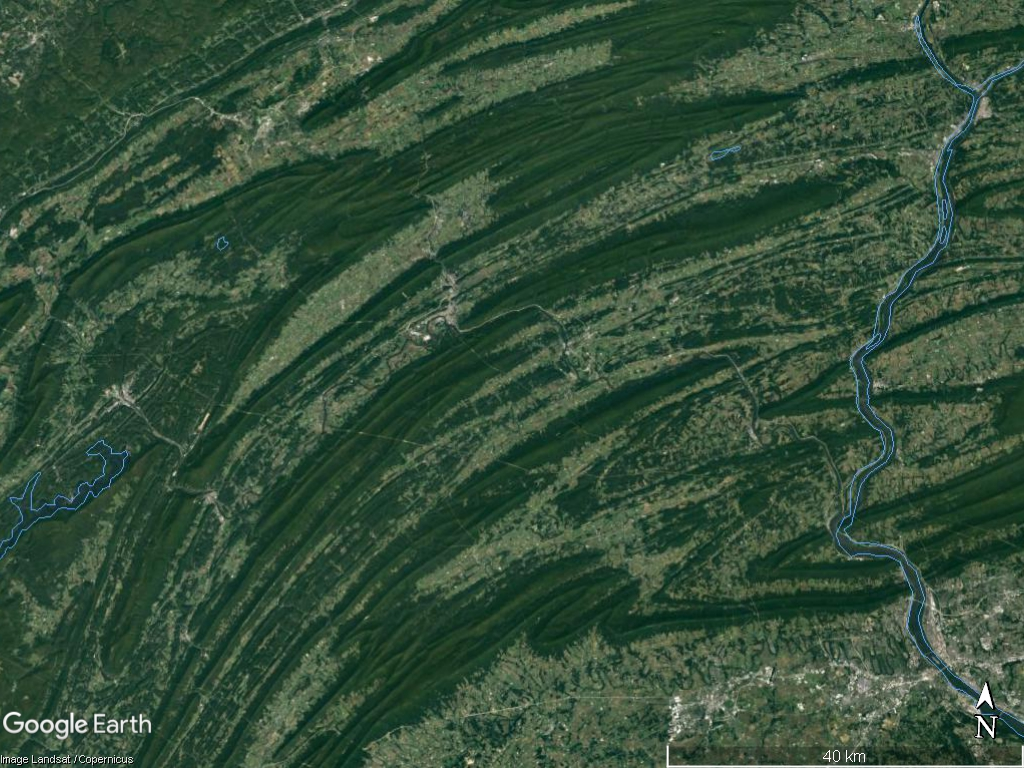
\includegraphics[width=1\linewidth]{obrazky/tectonic/apalachian}
	\caption{Apalačské pohoří v USA (zdroj Google Earth)}
	\label{fig:apalachian}
\end{figure}

Velice často je s vrásami spojená tzv. \emph{inverze reliéfu}. Horniny v ose antiklinály jsou značně tektonicky porušené (rozpukané), jsou tedy i náchylnější k erozi. Dlouhodobým vývoje reliéfu dochází k oderodování antiklinály a vzniku \emph{antiklinálního údolí}. Elevace jsou tvořeny synklinálou.

\section{Strukturní reliéf}

\begin{figure*}[h]
	\centering
	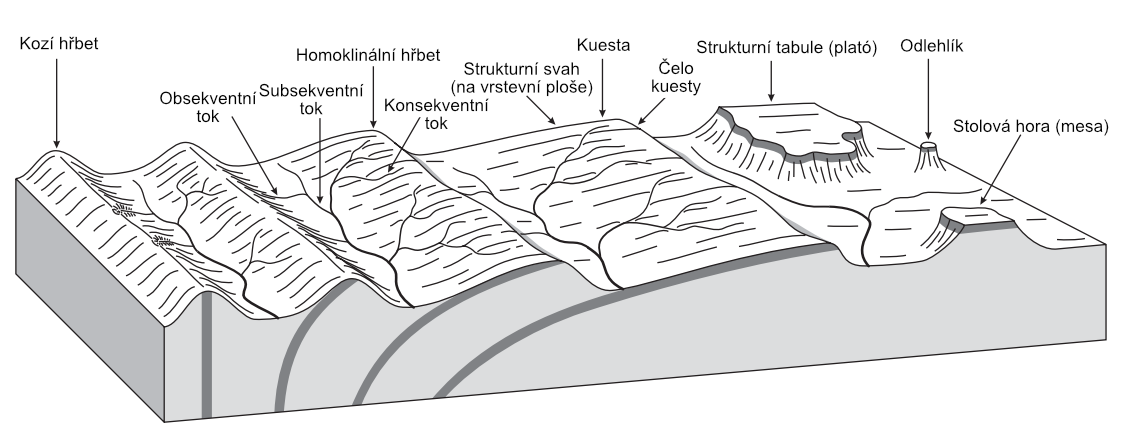
\includegraphics[width=1\linewidth]{obrazky/tectonic/strukturni_tvary}
	\caption{Strukturní reliéf -- tvary na horizontálních a ukloněných vrstvách. Horizontální vrstvy -- strukturní tabule, stolová hora a odlehlík. Ukloněné vrstvy -- kuesta, homoklinální hřbet a kozí hřbet. Označené jsou i základní typy vodních toků. Konsekventní -- ve směru sklonu vrstev, subsekventní -- po směru vrstev a obsekventní -- proti směru sklonu vrstev. Tmavě šedé pásy vyznačují polohz odolných hornin (upraveno podle \textcite{huggettFundamentalsGeomorphology2007}).}
	\label{fig:strukturnitvary}
\end{figure*}

\subsection{Horizontálně uložené vrstvy}
Sedimentární horniny, které nebyly postižené vrásněním mají zpravdila horizontálně až subhorizontálně uložené vrstvy. 
Fluviální erozí a svahovými procesy se v takovýchto oblastech vyvíjí \emph{strukturní tabule} (\enquote{plateaux)}, což jsou rozsáhlé ploché elevace, které jsou od svého okolí oddělené strmými svahy. Postupným rozrušováním tabule vznikají plošně menší \emph{stolové hory} (\enquote{mesa}), \emph{svědecké vrchy} až \emph{odlehlíky} (\enquote{butte}) a úzké a vysoké \emph{skalní jehly} (\enquote{pinnacles)}. Důležitou podmínkou je přítomnost odolnějších hornin v nadloží (\enquote{caprock}), které brání celkové erozi (Obr. \ref{fig:strukturnitvary}).

V oblastech, kde je časté střídání tvrdých (odolných) a měkkých (málo odolných) vrstev, se vyvíjejí \emph{strukturní stupňoviny}. Kdy odolné vrstvy tvoří stupně -- \emph{strukturní terasy}.

\subsection{Ukloněné vrstvy}
Na ukloněných horninách (do \SI{7}{\degree}), které mají různou odolnost, se vyvíjejí asymetrické hřbety -- \emph{kuesty} (Obr. \ref{fig:strukturnitvary}). Čelo kuesty je strmé a vzniklo erozí ukloněných vrstev. Týlní svah je mírný a odpovídá sklonu vrstev (\enquote{dipslope}). Kuesty se často nacházejí ve skupinách a jejich počet odpovídá počtu odolných vrstev. 

Při větším sklonu vrstev (\SIrange{7}{40}{\degree}) vznikají asymetrické hřbety označované jako \emph{homoklinální}. Při sklonu nad \SI{40}{\degree} pak \emph{kozí hřbety}, které mohou být v příčnem profilu již symetrické (Obr. \ref{fig:strukturnitvary}).

